\documentclass[tikz,border=6pt]{standalone}
\usepackage[T1]{fontenc}
\usepackage[utf8]{inputenc}
\usepackage{helvet}
\renewcommand{\familydefault}{\sfdefault}
\usepackage{xcolor}
\usetikzlibrary{arrows.meta}
\definecolor{cblue}{HTML}{1F4E79}
\definecolor{cgreen}{HTML}{2E7D32}
\definecolor{cred}{HTML}{C62828}
\definecolor{cgrey}{HTML}{808080}
\definecolor{paleblue}{HTML}{E8F0F8}
\definecolor{palegreen}{HTML}{E8F5E9}
\definecolor{palered}{HTML}{FFEBEE}
\definecolor{palegrey}{HTML}{F5F5F5}
\begin{document}

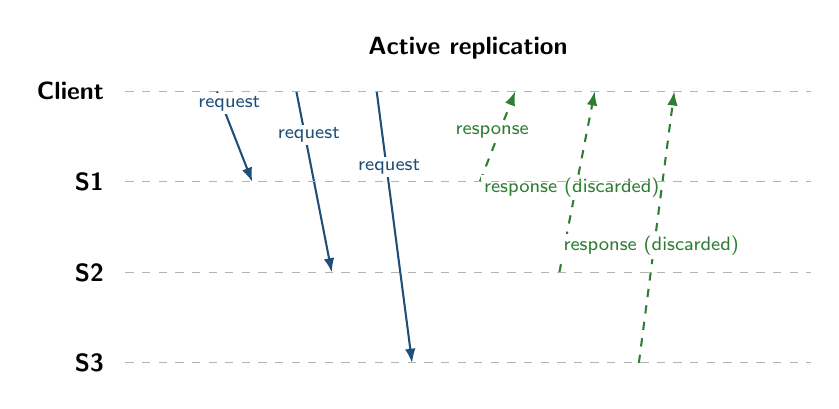
\begin{tikzpicture}[x=1cm,y=1cm]
\node[font=\small\bfseries] at (4.35,0.55) {Active replication};
\draw[-{Latex[length=1.8mm]},cblue,solid,line width=0.75pt] (1.16,0.000) -- (1.61,-1.150) node[pos=0.35,above,yshift=3pt,fill=white,inner sep=1pt,font=\scriptsize] {request};
\draw[-{Latex[length=1.8mm]},cblue,solid,line width=0.75pt] (2.17,0.000) -- (2.62,-2.300) node[pos=0.35,above,yshift=3pt,fill=white,inner sep=1pt,font=\scriptsize] {request};
\draw[-{Latex[length=1.8mm]},cblue,solid,line width=0.75pt] (3.19,0.000) -- (3.64,-3.450) node[pos=0.35,above,yshift=3pt,fill=white,inner sep=1pt,font=\scriptsize] {request};
\draw[-{Latex[length=1.8mm]},cgreen,dashed,line width=0.75pt] (4.50,-1.150) -- (4.95,0.000) node[pos=0.35,above,yshift=3pt,fill=white,inner sep=1pt,font=\scriptsize] {response};
\draw[-{Latex[length=1.8mm]},cgreen,dashed,line width=0.75pt] (5.51,-2.300) -- (5.96,0.000) node[pos=0.35,above,yshift=3pt,fill=white,inner sep=1pt,font=\scriptsize] {response (discarded)};
\draw[-{Latex[length=1.8mm]},cgreen,dashed,line width=0.75pt] (6.52,-3.450) -- (6.97,0.000) node[pos=0.35,above,yshift=3pt,fill=white,inner sep=1pt,font=\scriptsize] {response (discarded)};
\draw[cgrey!60,line width=0.4pt,dashed] (0,0.000) -- (8.7,0.000);
\node[anchor=east,font=\small\bfseries] at (-0.15,0.000) {Client};
\draw[cgrey!60,line width=0.4pt,dashed] (0,-1.150) -- (8.7,-1.150);
\node[anchor=east,font=\small\bfseries] at (-0.15,-1.150) {S1};
\draw[cgrey!60,line width=0.4pt,dashed] (0,-2.300) -- (8.7,-2.300);
\node[anchor=east,font=\small\bfseries] at (-0.15,-2.300) {S2};
\draw[cgrey!60,line width=0.4pt,dashed] (0,-3.450) -- (8.7,-3.450);
\node[anchor=east,font=\small\bfseries] at (-0.15,-3.450) {S3};
\end{tikzpicture}
\end{document}
